\documentclass[11pt]{article}

\usepackage{a4wide}
\usepackage{mathptm}
\usepackage{xspace}
\usepackage{amsmath}
\usepackage{graphicx}
\usepackage{algorithm}
\usepackage{algpseudocode}
\usepackage{tikz}
\usepackage{tkz-graph}
\usetikzlibrary{shapes.misc, positioning}
\usepackage{listings}
\usepackage{color}
\usepackage{xcolor}
\usepackage{hyperref}

\definecolor{dkgreen}{rgb}{0,0.6,0}
\definecolor{gray}{rgb}{0.5,0.5,0.5}
\definecolor{mauve}{rgb}{0.58,0,0.82}

\lstset{frame=tb,
  language=Java,
  aboveskip=3mm,
  belowskip=3mm,
  showstringspaces=false,
  columns=flexible,
  basicstyle={\small\ttfamily},
  numbers=left,
  numberstyle=\tiny\color{gray},
  keywordstyle=\color{blue},
  commentstyle=\color{dkgreen},
  stringstyle=\color{mauve},
  breaklines=true,
  breakatwhitespace=true,
  tabsize=3
}
\begin{document}

\title{Report SpringApp Project Group 4}

\author{Jacek Antoni Wegrzynowski, Rashaad Wells Iversen, Veronicha C. T. Pettersen }

\maketitle

\begin{abstract}

\noindent \textit{This document describes the journey of a group of students at Western Norway University of Applied Sciences took to develop a web-based application prototype to create poll and receive votes.  The prototype's creation involved a new learned technology stack, integrating Angular, Spring Boot, JPA, Hibernate, H2, MQTT and Java.  We achieved significant functionalities, including user registration and authentication, poll and question creation, poll searching, and versatile voting mechanisms via both web interface and IoT integration.  Remarkably, these milestones were reached despite the team's initial lack of Java expertise, demonstrating a commendable learning curve and adaptability.  The successful implementation of these features showcases the prototype's potential to deliver a final product for polling.  While the complexity of our work may not align with every expectation, we take considerable pride in the achievements we have realized.  Our efforts reflect significant dedication and learning, particularly in areas initially unfamiliar to us.}

\end{abstract}

%\input{commands}

\section{Introduction}
\label{sec:introduction}

This document outlines the development of a web-based application designed to facilitate interactive polling and voting processes. The application prototype was developed to meet specific requirements for the group project.

\begin{itemize}
\item Web Front-End: The application will feature a user-friendly web front-end, enabling users to interact with the system via a web browser. This interface will serve as the primary point of user interaction for conducting polls and voting.

\item Business Logic Implementation: Essential business logic will be embedded within the application to handle the processing of polls, votes, user interactions, and other related functionalities.

\item REST API: The application will include a RESTful API, exposing a select subset of the business logic. This API will facilitate external interactions and integrations with the application.

\item Database Integration: Persistent storage of polls, voters, users, and other relevant entities will be managed through a relational database, ensuring data integrity and consistency.

\item Voting and Display Device: The project encompasses the development of a voting and display device, which may be either virtual or physical. This device will interact directly with the application's business logic and contribute to the polling process.

\item Publish-Subscribe System Integration: Results and outcomes of polls will be disseminated through a publish-subscribe messaging system, enhancing the reach and accessibility of polling data.

\item Dweet.io Integration: Key events such as the initiation and conclusion of polls, along with pertinent information, will be published to dweet.io using RESTful services, ensuring real-time updates and public accessibility.

\item Analytics Component: An analytics subsystem will be implemented, tasked with subscribing to poll data and storing results in a NoSQL database. This component will enable advanced data analysis and insight generation.

\item Security Considerations: The application will be developed with a strong focus on security aspects, including confidentiality, authentication, and authorization, to protect user data and ensure system integrity.

\item Cloud Deployability: While the application will be designed for cloud deployment, actual deployment to a cloud environment is not a mandatory requirement of this project.
\end{itemize}

\noindent The development of this application aims to integrate these requirements into a single system allowing an interactive polling and voting environment.\\


\noindent The technology stack for this project includes a variety of frameworks and systems, each in response to specific aspect of the application's functionality. For the front-end development, we have used Angular to create a responsive and interactive user interface. The business logic and backend services are powered by Spring Boto. To manage the data, we utilize JPA for our relational database needs, ensuring effective data management and retrieval, while H2  is employed for non-relational database operations, offering flexibility and scalability on a Hibernate database. Additionally, Mosquitto is the chosen messaging system, facilitating reliable and efficient message handling across different parts of the application. \\

\noindent In the prototype implementation of our application, we successfully achieved several key functionalities, crucial for its operation and user engagement. The prototype allows for user registration, enabling new users to create accounts and gain elevated access. Once registered, users can seamlessly log in and log out, ensuring secure access to their profiles and activities. A significant feature of the prototype is its capability to create polls, allowing users to initiate new voting sessions. In addition to this, users can also create unlimited questions within these polls. The system includes a feature to search for and find specific polls. \\

\noindent Voting mechanisms have been implemented in two distinct forms: users can cast their votes through the web interface, providing ease of access and convenience and/or  have the functionality to cast votes via an IoT device, showcasing the application's capability to interface with physical hardware for a more interactive polling experience.  The prototype successfully demonstrates a few aspects of the creation of a web application with the ability to perform CRUD operations and handle user authentication.  API testing with Postman, demonstrates the application to be responsive and functional. The prototype's functionality, achieved under these circumstances, thus not only showcases the application's capabilities but also reflects the team's dedication and skill in overcoming technical challenges.\\



\noindent In this document, we have started with this introductory section where we explain the background and context of the assignment, setting the stage for an understanding of the objectives of the project.  Second, provide an overview of our technology stack, including a breakdown of each technology's role and purpose in section~\ref{sec:technology}.  Next, we provide an in-depth explanation of the system architecture and design, detailing how we planned to build our project in section~\ref{sec:design}.  This is followed by section~\ref{sec:implementation}, an explanation on how we actually implemented the our ideas, including code snippets on topics we found specifically interesting to describe in depth.  Furthermore in section~\ref{sec:evaluation}, we describe testing methodologies and experiments used to ensure the functionality of the application performed as expected.  Section ~\ref{sec:conclusion} concludes the report, presenting a reflective overview of our journey through this project. This section boasts our achievements, discusses the challenges and lessons learned from this experience, offers a candid appraisal of our overall teamwork, and expresses our sentiment towards missed opportunities.



\section{Software Technology Stack}
\label{sec:technology}

\textcolor{red}{Introduce in (sufficient) depth the key concepts and architecture of the chosen software technologies. As part if this, you may consider using a running example to introduce the technology.}

\textcolor{red}{Emphasize the “new” software technologies that was selected by the group and which has not been covered in the course.}

\textcolor{red}{This part and other parts of the report probably needs to refer to
figures. Figure~\ref{fig:framework} from \cite{brown:96} just
illustrates how figure can be included in the report.}

\subsection{Angular:}
We chose Angular as our web application framework to develop the frontend of the FeedApp
prototype. Angular is a popular, open source TypeScript based framework\footnote{1} that is used to create
Single Page Applications (SPAs). SPAs are web applications that only loads one single page, and then
changes the content of that page depending on how the user interacts with the page.

\subsubsection{Fundamental Consepts of Angular }
\begin{itemize}
\item Components: Components are many places described as the main building blocks for Angular applications. Each
component will contain one HTML-file with the UI-template of the component and one TypeScript-
file that contains the components logic. It can also contain CSS or SCSS files, defining the styles of the
component, as well as test files and configuration files. A component defines a specific view, as well
as the functionality that goes into that view. In other words, it contains both what the user sees in
the UI and the logic that goes into the component.
\item Services: It is also possible to share different functions and logic between different components. This
can be done by creating a service, which is a TypeScript file that is used for tasks such as for example
business logic and handling of data. In our FeedApp implementation, we created services dedicated to managing authentication and handling poll data.
\item Dependency Injection (DI): Services can also be used to inject dependencies into multiple
components, with the use of DI. This is useful for connecting the different parts of the application.
\item Routing: The Angular Router handles the navigation between different views as users performs different tasks. This is a key element in SPAs since instead of reloading the page every time the view is changed.
\end{itemize}

One of the main advantages of creating the application as a SPA is that it speeds up the development
process.
For more 
Resourses used for writing this paragraph: https://angular.io/guide/architecture 

\subsection{Spring Boot}
\label{subsec:springboot}

We have chosen Spring Boot as our enterprice software framework when developing our application. Spring Boot is an extension of the Spring Framework that simplifies the development process, making it possible to create a functioning web application fast. Considering the time limitation we had on our project, Spring Boot seemed like a good choice when choosing a framework. 

\subsubsection{Spring Framework}

To fully understand the benefits of the Spring Boot extension, we are first going to briefly go through some core concepts in the Spring Framework\footnote{2}:

\begin{itemize}
    	\item Bean Definition: Beans are often described as the backbone of a Spring application. They are managed by the Spring Inversion of Control (IoC) Container. How they are configured, and how their lifecycle is managed plays an important role when having a smooth and proper running application. 
    \item Dependency Injection (DI): Spring's DI mechanism manages dependencies among application components. This setup is crucial for injecting required services and modules into different parts of the application.
    \item Aspect-Oriented Programming (AOP): In Spring, AOP makes it possible to handle tasks that are common in multiple parts of an application efficiently by defining the function and then applying it to the sections that need to use it.
\end{itemize}

How a Spring application is deployed:

\begin{itemize}
    \item Packaging: The application is compiled and packaged, typically into a JAR or WAR file, ready for deployment.
    \item Running on a Server: The packaged application is deployed on a web server. Spring Boot, with its embedded server capability, simplifies this by allowing the application to run independently without needing a separate server setup.
\end{itemize}

\subsubsection{Spring Boot's Role in FeedApp:}
\begin{itemize}
    \item Auto-Configuration: Spring Boot automatically configures the application based on the included libraries, reducing the need for extensive manual configuration.
    \item Simplified Deployment: The embedded server feature of Spring Boot allows our application to be deployed as a standalone unit, enhancing ease of deployment and portability.
\end{itemize}

In the implementation of our FeedApp prototype, the use of Spring Boots auto configuration and deployment functionalities has made it possible for us to spend more time on the applications business logic. 

\subsection{JSON Web Tokens}
\begin{itemize}
 \item We used an open standard called JSON Web Tokens (JWT), that provides a condensed, self-contained method for securely exchanging data as a JSON object between parties. This data is digitally signed, so it can be validated and trusted. RSA or ECDSA can be used to sign JWTs with a secret key or a public/private key pair. \footnote{https://datatracker.ietf.org/doc/html/rfc7519}
 \item JWTs are essential to our FeedApp's authentication procedure. A JWT is given to a user upon login. Subsequent requests to authenticate the user and grant access to restricted routes, services, and resources within the application will then utilize this token. Because of their short size and ease of use, JWTs are the ideal format for our application and work well in our web-based environment.
\end{itemize}

\subsection{H2 Database}
\begin{itemize}
 \item We used a quick and easy approach to store and manage data with the lightweight H2 database. Because of its cheap overhead and ease of setup, it's especially helpful throughout the development and testing phases. H2 can operate embedded within a Java program or in client-server mode.
 \item We are using the H2 database in FeedApp development for testing and prototyping. It eliminates the requirement for a complicated database setup and enables us to simulate database interactions and run unit tests. The H2 database is the perfect option for our needs for rapid development because it interfaces with our Spring Boot platform.
\end{itemize}

\subsection{Hibernate}
\begin{itemize}
 \item For Java applications, Hibernate is a powerful Object-Relational Mapping (ORM) framework. It offers a framework for converting a conventional relational database to an object-oriented domain model. Hibernate resolves the mismatch issues by substituting high-level object handling routines with direct, permanent database accesses. \footnote{https://hibernate.org/orm/}
 \item Hibernate is used in our FeedApp to make it easier for our Java application to communicate with the database. The CRUD (Create, Read, Update, Delete) procedures are made simpler and more effective by managing database operations and data persistence. Our team is able to concentrate more on the business logic and less on database management because Hibernate abstracts the database logic.
\end{itemize}

\subsection{Java Persistence API}
\begin{itemize}
 \item A Java specification for managing, retrieving, and storing data between Java objects and a relational database is called the Java Persistence API (JPA). JPA, which is a component of the Java EE platform, makes it easier to create Java apps that communicate with databases.
 \item JPA is implemented into FeedApp to manage our application's relational data. It offers a platform for managing relational data in Java programs and executing database operations on Java Entities. Hibernate and JPA work together to make database administration in our application more error-free and efficient.
\end{itemize}

\subsection{Mosquitto MQTT}
\begin{itemize}
 \item A simple publish-subscribe network protocol called MQTT (Message Queuing Telemetry Transport) is used to send messages between devices. Mosquitto is portable and works with a wide range of devices, including powerful servers and single-board computers with minimal power consumption. \footnote{https://mosquitto.org/}
 \item Mosquitto MQTT is essential to our FeedApp since it manages real-time messages and facilitates effective connectivity with IoT devices. MQTT is a good solution for our IoT-related capabilities since it guarantees efficient and reliable message delivery even in limited contexts. Maintaining the application's responsiveness and performance requires minimal resource usage, which is ensured by its lightweight design.
\end{itemize}

\begin{figure}
  \centering
  \includegraphics[scale=0.5]{figs/framework.png}
  \caption{Software technology evaluation framework.}
  \label{fig:framework}
\end{figure}


\clearpage
\section{Design of the FeedApp Prototype}
\label{sec:design}

\subsection{Architectural Overview} 

Our fundamental idea of the FeedApp application was to mimic some of the Kahoot application capabilities while remaining simplistic, keeping alignment with good practices \footnote{Code Complete: A Practical Handbook of Software Construction, Second Edition } in software development and prototyping.  Our archtiecutre aims to meet requirements, demonstrate core functionality, and balance the effort put into development of a prototype.  \\

\noindent The application is accessible through web browsers, ensuring compatibility with devices such as smartphones, tablets, and computers.  The application provides registered users with the ability to create and participate in various polls.  It offers the flexibility for users to cast their votes using either a physcial IoT device or through a web browser.  The application incorporates a user authentication system, ensuring secure access and protecting user identities and information.

\subsection{Domain Model} 
Our domain model of the FeedApp, is represented in a Unified Modeling Language (UML) class diagram representing the fundamental objects and their relationships. By doing this we describe  behavior and functions in a clear way so that we are all on the same page.  Throughout the development lifecycle of the FeedApp, this domain model has undergone iterative modifications. These adaptations were essential to maintain alignment with changes made in our objectives.  A primary focus during these modifications has been the preservation of simplicity within the system's architecture. By continuously refining the domain model, we have ensured that the FeedApp remains functionally efficient.

\subsubsection{Users}
The domain model describes an entity of a user and categorizes it into two distinct types based on account registration status.  Users with registered accounts are granted full access within the FeedApp including the capability to create and participate in both public and private polls.  This category of user must undergo an authentication process which is described in TODO:Section.  Users without registerd accounts are only allowed to participate in publicly accessible  polls.  This restriction is a delibarate choice, allwoing our development efforts to maintain simpliciy in implementation.  

\subsubsection{Polls}
A key feature of the system is the poll entity, characterized by distinct attributes such as a title, an identification number, and the option to be set as private or public. Each poll is required to have a time limit and are also designed to integrate with Internet of Things (IoT) devices.  Furthermore, polls are designed to be flexible, allowing an unrestricted number of questions. The application does not impose a limit on the quantity of questions per poll.  In addition to this, for private polls, there is a feature to specify a list of authorized users who are permitted to vote. 
In the design of polls, the questions must be structured as binary-choice and closed-ended.  This format restricts responses to one of two predetermined options, exemplified by pairs such as True/False, Yes/No, or Pancakes/Waffles.  While the application does not impose time limits on individual questions, it integrates time restrictions at the poll level.  This design choice, made for ensuring simplicity in implementation, focuses on the entire poll rather than individual questions.

\subsubsection{IOTDevice}
For this project, a physical IoT device was chosen to add the interactive dimension to the polling process.  This device is intentionally simplistic, capable only of transmitting voting data without knowledge of the specific poll or question involved.  It operates via a Mosquitto broker, which relays messages from the IoT device to the feed application. The integration with the IoT device is minimalistic. The device's primary function is to acknowledge a voting action and communicate this to the feed application. It is not equipped to discern details about the poll or the voting options. The absence of an on-device display is compensated for by using a command-line interface to indicate when a vote has been cast. This setup was demonstrated in the submitted video, showcasing the Mosquitto broker's role in facilitating communication between the IoT device and the feed application.

\subsubsection{IOTDisplay}
The project's infrastructure includes an Internet of Things (IoT) device, functioning independently on a dedicated hardware platform. This device establishes a wireless connection with a Windows-based HP laptop, which serves a dual purpose: as a control unit and as a display for the IoT device's operations. The design stipulates that both the IoT device and the laptop must share the same Wi-Fi network for seamless communication.

\subsubsection{IOTDevice Integration with FeedApp}
Further enhancing the system's architecture is the incorporation of a Linux virtual machine (VM) on the HP laptop. This VM is designated as the application server, managing the core functionalities of the feedback feed application. Notably, the VM's connectivity is not restricted to the same Wi-Fi network as the IoT device, offering flexibility in network configurations. It communicates with the IoT device through a Mosquitto broker, which acts as an intermediary in message transmission. The IP address of the Mosquitto broker is hardcoded into the system for consistent connectivity.\\

\noindent Messsage sent from the IoT device are sent via Transmission Control Protocol (TCP) to the Mosquitto Broker. When a user interacts with the IoT device, by pressing a button, this action triggers a message that is relayed by the Mosquitto broker then pushblises the message to all of it's subscribers. The MQTT receiver  is responsible for subscribing to the IOT messages and then sending the HTTP post representing the button push.  The application IOTController is configured to recognize this inpu and then triggering logic to determine the active poll and the specific question being addressed by the IoT device. While the mechanism for transitioning between different poll questions was not fully established, the design suggests that the REST API would facilitate this progression by incrementally recording votes and navigating to subsequent questions.

\subsubsection{Analytics}
Once the a vote is cast on the last quesiton in the poll, the application is designed to immediately reflect the analytical data offering insight into collective responses.  The system is designed to facilitate the display of analytics for all polls, regardless of their current status (active or inactive).  This functionality is implemented through a standardized display template, which is accessible via web browsers. The template ensures uniformity in the visualization of analytics, providing a coherent and consistent user experience. In addtion, the system's architecture allows for third-party applications to access poll-related data.  This capability enables external entities to conduct their own analytical assessments.  However, it is important to note that the scope of data accessible to third-party applications is confined to poll-level information. Granular data pertaining to individual questions within the polls is not available for external analysis.

\subsection{FrontEnd Design} 
To get an overview of how we wanted to implement the user interface, an application flow diagram was modeled. 
The diagram displays how the user navigates through the different frames in the front end of the application: \\

\begin{figure}[h]
  \centering
  \includegraphics[scale=0.30]{figs/Application Flow Diagram (1).png}
  \caption{Application Flow Diagram}
  \label{fig:appFlow}
\end{figure}


\noindent Each screen has in the diagram been modelled as a state, and for every state, the user is able to do some action or provide some input. 
These actions or inputs are modelled as transitions, and are in the figure above illustrated with arrows. Transitions that results in errors are 
colored red, and transitions that does not result in errors are colored green. Our application consists of six screens. We have a login screen, 
where the user can either login, or create a new user. Once the user is logged in, he is directed to a start screen, where he gets the option to 
do multiple actions. He can search for a poll, which then can be voted on, or he can view and manage his own polls. He can create new polls,
and in this state he gets the option to pair the poll with an IoT device. \\


\clearpage
\section{Prototype Implementation}
\label{sec:implementation}

\subsection{Frontend}
The following components have been implemented for the front end:

\begin{itemize}
	\item Login: this is the first view that the user are presented with. It’s main purpose is to
authenticate users, and help them access the application. It contains input fields for
username and password. When the user presses “Log in”, he is taken to the main-page of the
application. If the user is not registered, he can easily do so by pressing the “Register”-
button.
	\item Register: here the user is presented a schema, where he can register and that way access the
application. He needs to add an email address, a username and a password. Once the
information is submitted, the user is sent back to the login page.
	\item Main-page: This component contains buttons that lets the user easily navigate to all parts of
the application quickly.
	\item Find-poll: Here the user can search for a poll via its id, or by a poll-name. All the polls that
matches the input will then be displayed with the option to vote on it.
	\item Create-poll: Here the user can create a new poll. He can decide the questions that should be
displayed, when the poll is active, if it is private and invite users to participate in it. Once
created, a poll-id is given to the user. This can for example be given to other users and used
to search for the poll.
	\item Vote: Here the user gets to submit votes to active polls.
\end{itemize}

\noindent A authentication service, a poll service and a voting service has also been created to handle logic that
can be applied to multiple components. The authentication service handles operations such as
logging the user in to the application and searching for users. The poll service handles logic depicting
the polls such as finding polls, creating polls and changing polls. The Voting service handles the logic
connected to the voting.  The following subsection describes more detailed how the logic behind the authentification process has been implemented, 
and displays how the frontend is connected to the REST API. 

\subsubsection{Authentication Process}
A crucial part of the frontend implementation is the user authentication process. 
This is managed through the \texttt{login} method in the \texttt{auth.service} file and the \texttt{onSubmit} method in the \texttt{LoginComponent}.  The \texttt{login} method is defined as: \\

\begin{center}
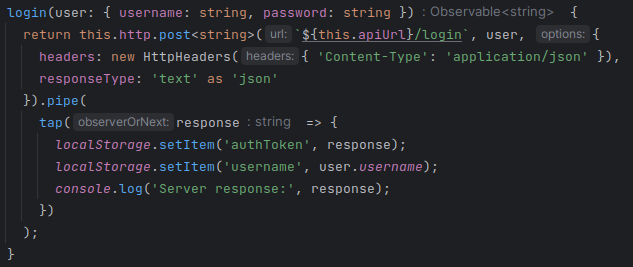
\includegraphics[width=0.80\textwidth]{figs/login.png}
\end{center}

\noindent This method handles user login credentials, sending them to the backend for verification and storing the received token and 
username in the browser's local storage for session management. The token is stored in the local storage to maintain the user sessions. \\

\noindent The \texttt{LoginComponent} uses this service in its \texttt{onSubmit} method: \\

\begin{figure}[h]
  \centering
  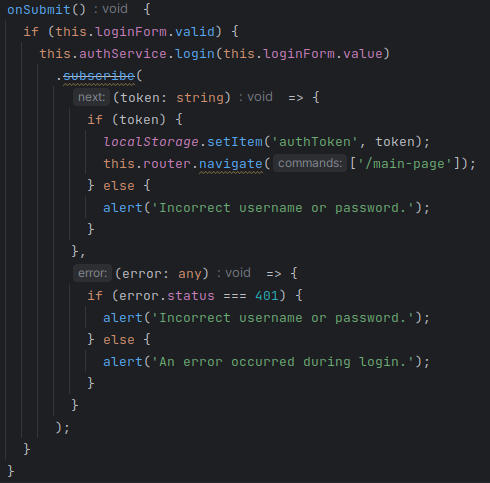
\includegraphics[width=0.80\textwidth]{figs/on_submit.png}
  \caption{Verification Service Example}
  \label{fig:my_label}
\end{figure}

\noindent This function makes sure that only users with valid credentials are able to access the main page of the application, while also handling 
different error scenarios. If a user gives an incorrect credential or any other login error occurs, an error message is displayed. \\

\subsection{Backend}
The architecture of our program has modular architecture that includes multiple important entities and their corresponding repositories.

\subsubsection{Entities}
We will begin by describing the structural components of the application which is object-oriented by design. The primary class, \texttt{AppUser}, implements properties such as username, email, and password. It also holds a collection of polls owned by the AppUser.  A critical feature of this class is the implementation of two-factor authentication, validated through a verification code to ascertain user authenticity. \\

\noindent The \texttt{Poll} class, a core entity in our application, represents polls created by users. It includes details like title, open/close status, and duration, and can contain multiple questions. The poll implements general properties for storing privacy status, activity status, duration, and IoT device pairing. It also implements specific properties like the poll title, vote tallies, a list of authorized users (for private polls only) and funttion implementation to perform question management such as add, delete and edit. Polls are also linked to IoT device and therefore, holds information on which device it is paired with.\\

\noindent The \texttt{Question} class constitutes individual items within polls for users to vote on. Records responses and associates with specific polls.\\

\noindent A \texttt{Vote} class records user votes in polls, indicating 'yes' or 'no' choices. It contains the logic that is responsble for determining which question in a poll the vote should be submitted towards.\\

\noindent The \texttt{IoTDisplay} is a singleton class only aware of its associated IoT device by the property pariedDevice, which contains a string value of of the device name. \\

\noindent \texttt{ThirdPartyApp} interface class provides logic to allow third party entties to retreive data from the application. \\


\subsubsection{Repositories}
JPA repositories helps with performing create, read,update and delete (CRUD) database operations by reducing the need to manually code complex SQL queries.  We use these repositories with JPA EntityManager to interact with the database. We have defined various repositories in the FeedApp responsible for handling specific data operations.\\

\noindent The \texttt{AppUserRepository} manages the \texttt{AppUser}entity data operations, including user lookup by username.
\noindent \texttt{PollRepository} handles data operations for the \texttt{Poll} entity, with custom queries for poll title searches.\\

\begin{figure}[h]
  \centering
  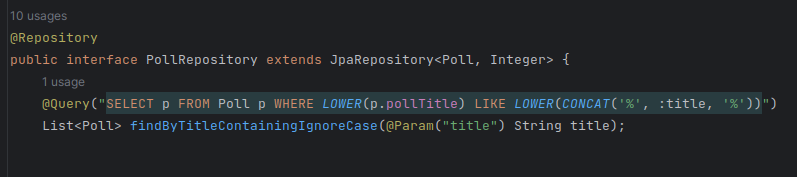
\includegraphics[width=0.80\textwidth]{figs/poll_repository.png}
  \caption{Custom Poll Title Query}
  \label{fig:my_label}
\end{figure}

\noindent The \texttt{QuestionRepository} provides data access for \texttt{Question} entity.
\noindent \texttt {VoteRepository} manages \texttt{Vote} data, including vote counting in polls.

\begin{figure}[h]
  \centering
  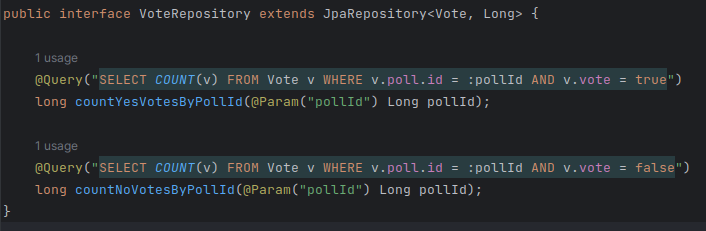
\includegraphics[width=0.80\textwidth]{figs/vote_repository.png}
  \caption{CustomVoting Query}
  \label{fig:my_label}
\end{figure}

\subsubsection{Integration with Spring Boot, Hibernate, and JPA}
In the implementation of our voting application, we employed several key technologies and tools including Spring Boot as the primary framework to simplify configuration and setup, Hibernate for Object-Relational Mapping (ORM) translation of Java object to database representations and JPA interfaces such as  \texttt{JpaRepository} for efficient data access and manipulation.


\subsubsection{Functionality}
In our application, we implemented several key functionalities including the he ability to register and manage user accounts, features for creating and managing interactive polls, voting mechanisms within these polls and Integration with a physcial IoT devices.

\subsection{REST API}
The web application consists of three key controllers, each handling different aspects of the voting system:

\begin{itemize}
    \item The AppUserController is responsible for user-related functions, including user authentication, registration, and the verification process.  It implements the AppUser entity using depencency injection by the @Autowired annotation to reference AppUserRepository and AppUserService. 
    \item The PollController oversees the management of polls, specifically handling the publication of poll results and controlling their status, whether open or closed.
    \item The QuestionController introduces and manages a voting mechanism for individual questions, reflecting a finer level of interaction and user engagement within the application.  It is mapped 
    \item The IOTController class in annotated with @RestController which is part of a RESTful web service in a Java application using the Spring Framework. It handles HTTP requests specifically related to IoT device notifications.  The controller is mapped to handle requests at the /api/notifications path.  It defines two endpoints for processing notifications sent from the IoT device, /api/notification/greenVote and /api/notification/redVote.  
\end{itemize}

\begin{figure}[h]
  \centering
  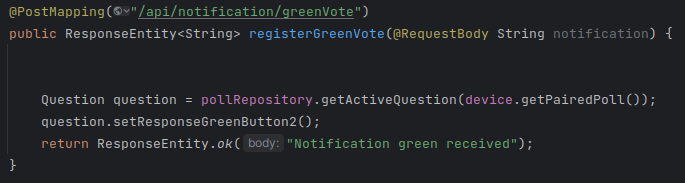
\includegraphics[width=0.80\textwidth]{figs/green_vote.png}
  \caption{Green Vote Endpoint}
  \label{fig:my_label}
\end{figure}

\noindent All controllers are designed following REST principles, offering a specific base URLs and using HTTP methods for standard CRUD operations.

\subsubsection{Spring Boot and Spring Data Integration}
They utilize Spring Boot's capabilities for creating standalone applications and Spring Data's repository pattern for data access. Dependency injection with \texttt{@Autowired} is also used.

\subsubsection{Error Handling and Response Management}
The controllers use \texttt{ResponseEntity} class for HTTP response handling, allowing them to manage different scenarios (even those ending with an error).  Method \texttt{deleteQuestion} in \texttt{QuestionController} that is responsible for deleting a question in a poll returns an error response if the question wasn't found:

\begin{figure}[h]
  \centering
  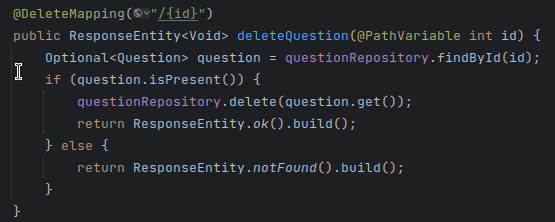
\includegraphics[width=0.80\textwidth]{figs/delete_mapping.png}
  \caption{Error Handling Response}
  \label{fig:my_label}
\end{figure}


\subsubsection{Security and User Management}
The \texttt{AppUserController} focuses on security and user identity management through authentication and JWT token management.  There are also a few features that we modelled into our application in the first phase of this project,
but due to the time constraints are yet to be implemented. These include Poll management and User
management. Currently the application allows users to create and participate in polls. However, the
management of the polls is not yet functional. The same goes for the management of the user
settings. The buttons has been created in the main-page component, but they are not directing the
users to new views yet.

\subsubsection{IoT Device}
The IoT device in our system is a physical unit and is implemented using C++ and the Arduino library\footnote{https://www.arduino.cc/reference/en/} and is based on the ESP8266 \footnote{https://www.nabto.com/esp8266-for-iot-complete-guide} module which includes Wi-Fi connectivity. This device is programmed with hardcoded Wi-Fi credentials which in our case is a cellar hotspot. Its design is straightforward, featuring just two buttons, referred to as the red and green buttons. The device is configured to publish a message to the MQTT broker whenever a button is pressed; however, it does not register continuous presses but only single clicks. These messages are then relayed by the MQTT broker, post distinct messages via REST interfacing with the IoTController.

  \begin{center}
  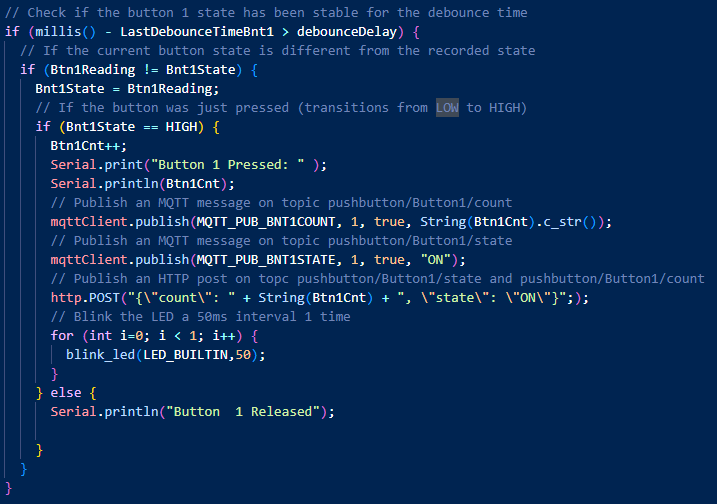
\includegraphics[width=0.80\textwidth]{figs/button1_pressed.png}
  \end{center}

\subsubsection{Messaging Receiver}
The MQTT message receiver is provided as a service in the voting application's Spring Boot backend.  It uses HTTP requests within the registerVote method to send votes to the voting applciation.  HTTP requests are asynchronous to ensure the other messages are not blocked.   While the current setup is sufficient for the purposes of a prototype application, it's important to note that for a product intended for release, a more secure implementation would be necessary.

  \begin{center}
  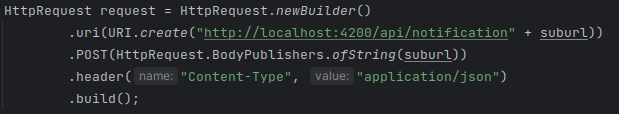
\includegraphics[width=0.80\textwidth]{figs/mqtt_publish.png}
  \end{center}

\subsubsection{Docker Container}
We created a Dockerfile in preparation for cloud deployment. This docker file invokes several events.  It builds the front end Angular application, build the Spring Bood back end application, sets an H2 database and then runs the applications.  

  \begin{center}
  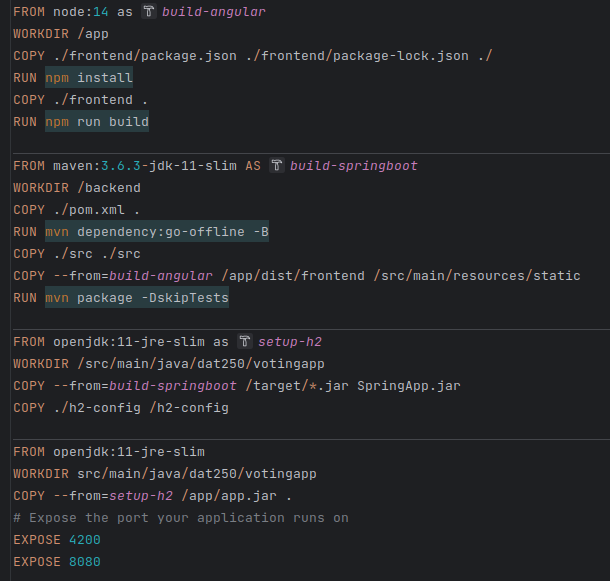
\includegraphics[width=0.80\textwidth]{figs/dockerfile.png}
  \end{center}

\section{Test-bed Environment and Experiments}
\label{sec:evaluation}

\subsection{Frontend testing}
When developing the frontend of our application, multiple testing strategies were performed to make sure that the 
application's functionalities were behaving as expected. One of the advantages of using Angular, is that it provides 
the option to do real-time compilation of the application. This feature made it possible to view the results immediately 
after code changes. This shortened the time spent on troubleshooting errors. The inspect tool in the browser were 
also a great tool that quickly let us inspect the applications. The console feature were handy when inspecting the 
HTML and CSS, and the Network analysis tool gave us a great insight into how the frontend and the backend 
communicated. Alerts were also created to notify the user whenever errors and issues occurred. 
of errors 

\subsection{JUnit testing}
The purpose of the JUnit tests is to verify our application's functionality. Using a mocking framework, they imitate particular application components, enabling targeted testing of individual functionalities without requiring the entire system. Important components analyzed are:

\begin{itemize}
    \item The ability of the application to successfully retrieve all items from a list, such as all users or polls.
    \item Capability to find a specific item by its unique identifier.
    \item Correct behavior of the application when an item cannot be found.
    \item The functionality to add, update, or remove items effectively.
\end{itemize}

Expected results, such as the quantity of objects recovered or the reaction in the event that an item is missing, are confirmed in each test. These tests are essential to ensure the application functions as expected.

\subsection{Postman testing}
Postman is a popular tool for testing REST APIs. It allows us to query the API endpoints of our application and receive back responses. The most important features tested using Postman include:

\begin{itemize}
    \item {Sending Different Types of Requests}: Postman test various request types like GET, POST, PUT, and DELETE. These are essential for operations in our application such as getting, creating, updating, or deleting data.
    \item {Verifying Responses}: The tool can verify whether the API returned the correct data and response codes. For instance, confirming that a GET request fetches the right list of items, or a 404 status code is returned when an item is not found.
    \item {Parameter Testing}: Postman allows testing how the API handles different parameters, such as specific item searches or result filtering.
    \item {Error Handling}: By sending incorrect or incomplete requests, we can test the API's error handling and check if it returns appropriate error messages.
\end{itemize}

\begin{figure}[h]
  \centering
  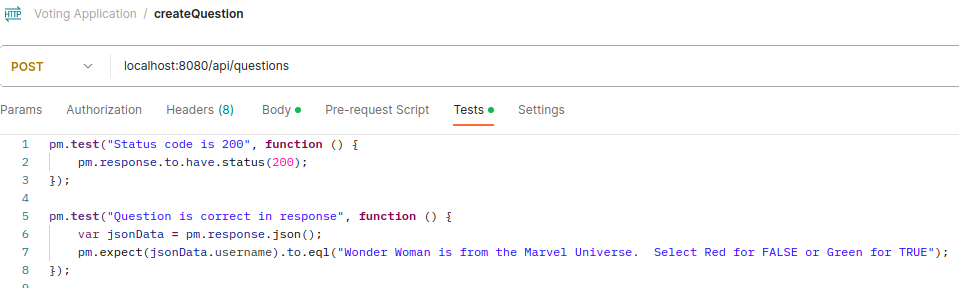
\includegraphics[scale=0.65]{figs/create_question_test.png}
  \caption{Sample Postman Test}
  \label{fig:appFlow}
\end{figure}

\noindent These tests make sure that our application's API is reliable, and performs as expected under different scenarios.

\subsection{IoT Device testing}

Testing of IoT device was testing using an informal and dynamic approach.  Instead of defining specific test cases, we relied on our domain knowledge, experience and creativity to find defects.  Using this type of testing allowed us to design, implment and test simultaneiously, enabling us to uncover design and development defects continiously in the software development loop. 

\clearpage
\section{Conclusions}

\noindent The overall design framework for the FeedApp project was pre-established at the beginning of the assignment. This design was further amplified through the course of various lectures that looked into different aspects of the project.  Given our initial unfamiliarity with many of the technologies outlined in the project's scope, we proceeded to adopt those specified in the project guidelines.\\

\noindent The project's brief did offer the option to incorporate one additional technology, which, while seemingly providing a degree of flexibility, also imposed certain constraints on our technological explorations. For example, questions such as the feasibility of implementing the project in Python, the use of a Python persistence model, or Python's capability to interface effectively with a database, remained unexplored. These potential avenues of inquiry could have provided a valabue alternative allowong a more complex design and quicker development approach.\\

\noindent However, the intensive and time-consuming nature of the assignments precluded a thorough investigation into these alternative technological possibilities. As a result, the project proceeded within the confines of the pre-specified technology stack, leaving some questions about potential alternative implementations and technologies unanswered.

\section*{References}
\begin{enumerate}
  	\item Angular Architecture Guide: \url{https://angular.io/guide/architecture }
	\item Spring Official Documentation \url{https://docs.spring.io/spring-framework/reference/index.html}
          \item JSON Web Tokens  \url{https://datatracker.ietf.org/doc/html/rfc7519/}
 	\item Hibernate ORM \url{https://hibernate.org/orm/}
	\item Mosquitto MQTT \url{https://mosquitto.org}
	\item Rapid Software Testing  \url{https://rapid-software-testing.com/}
\end{enumerate}

\section*{References}
\begin{enumerate}
	\item Angular Architecture Guide: \url{https://angular.io/guide/architecture }
	\item Spring Official Documentation \url{https://docs.spring.io/spring-framework/reference/index.html}
\end{enumerate}

\bibliographystyle{plain}
\bibliography{report.bib}{}

\end{document}
